% Figure 2: Multi-scale agency (Levin CLC) + Synthesis diagram — English

\begin{figure*}[!t]
\centering

\begin{minipage}[t]{0.48\textwidth}
\centering
{\small\bfseries C.\enspace Cognitive Light Cone (CLC)}\\[4pt]
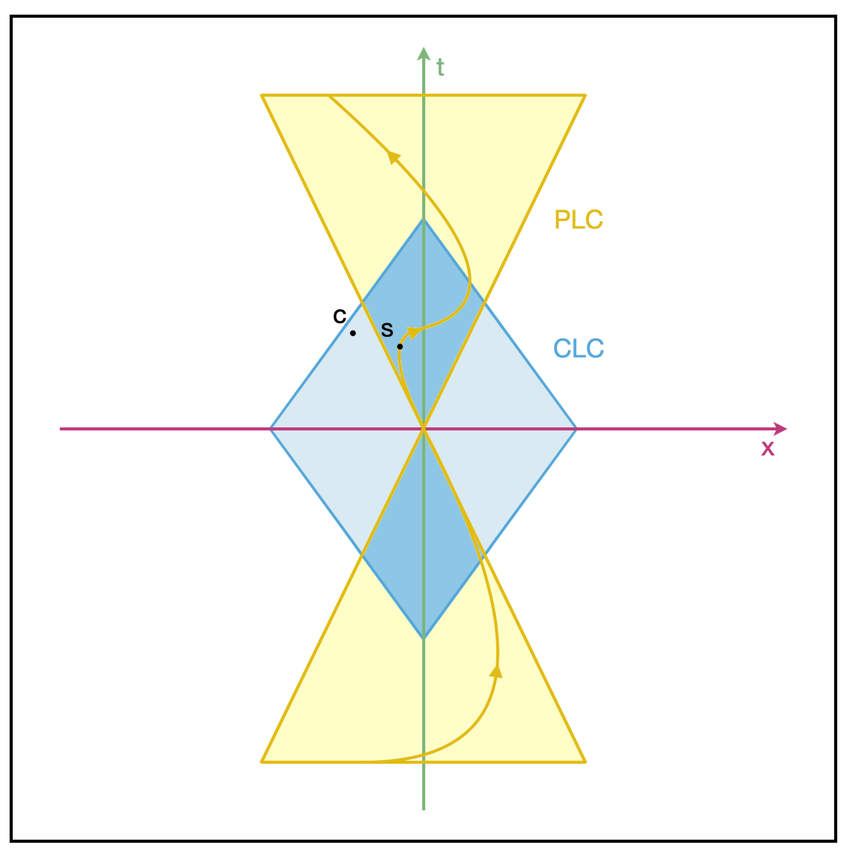
\includegraphics[width=0.85\textwidth]{figures/levin-clc-boundary.png}
\end{minipage}%
\hfill
\begin{minipage}[t]{0.48\textwidth}
\centering
{\small\bfseries D.\enspace The Synthesis}\\[4pt]
\includegraphics[width=0.85\textwidth]{figures/syntese_diag.png}
\end{minipage}

\caption{\textbf{C}: An agent's care light cone (CLC, blue) within the physical light cone (PLC, yellow). The care dimensionality $\dim C(A)$ determines which portion of the landscape the agent can represent. From \textcite{Doctor2024}. \textbf{D}: The synthesis equation: three source traditions converge on the core equation; dashed arrow shows $K$-expansion feedback.}
\label{fig:agency-synthesis}
\end{figure*}
